\section*{The Motivation Behind the Merge}
\addcontentsline{toc}{section}{The Motivation Behind the Merge}

This massively complex initiative to move the GPGPU onto the CPUs cores will provide huge advantages to programmers and computer designers in the future. These advantages in design and implementation result in more efficient programs, and an attempt at helping with the power wall. Briefly, the power wall is a result of performance scaling faster than power dissipation has. Simply put, faster computers are more difficult to keep cool.  

One of the big power draws in the system is the GPGPU sitting on the PCI-e bus. These huge cards draw a lot of power, and create a lot of heat. Besides powering (and cooling) the GPGPU core itself, the cards must cool the supplementary memory that the cards contain. Most of this energy spent on cooling the GPGPU will be alleviated by merging it onto the CPU. It can share the DRAM and cache with the CPU taking its own hot memory out of the equation. 

In addition to cooling the cards, the processor spends a lot of energy and time transporting all of the data the cards need. This can cause huge delays on the pipeline and tie up crucial buses. Moving the GPGPU onto the CPU can eliminate the time spent moving this data around. As mentioned previously, the GPGPU would share the memory infrastructure with the CPU allowing it easy access to any data it needs. 

Finally, the merge could bring great benefits to the programmer. Currently, while writing a program using CUDA or Open CL, the programmer must navigate an awkward interface to determine which parts of the program must be run on the GPGPU and reference the device (and track the reference) throughout the code. Hopefully, in a heterogeneous environment, the programmer could utilize a GPGPU with little or no effort. This could either be accomplished by the compiler, or through a process as painless as standard C pthreads. 

\section*{The Status Quo}
\addcontentsline{toc}{section}{The Status Quo}

Work has already begun in the space. Intel's Sandy Bridge \cite{tlpcache} and AMD's Fusion \cite{cpuassist} architectures moved the GPGPU form the north-bridge onto the CPU chip itself.\cite{tlpcache} This may have been for either cost saving reasons or for performance, but this represented a step in the march towards a heterogeneous architecture. Their fusion placed the GPGPU onto the die sharing a L3 cache and main memory. It however, is not, integrated into the CPU itself (as a heterogeneous architecture would be). Therefore, while the GPGPU and CPU have been integrated into the same chip, the programmer still writes code in the same way as before. In this model, the CPU will act as leader sending instructions, data, and code down to the GPGPU. 

Even still, this move is interesting because it pronounces some of the architecture questions around the integration between the CPU and the GPGPU. For one, how is the instruction set going to change? Will the CPU act as a leader dispatching instructions or will the compiler need to generate code specifically for the GPGPU core? For a completely efficient and effective heterogeneous architecture, the CPU cannot be expected to constantly lead the GPGPUs operations. That would force a bottleneck onto the CPU and require additional work on the CPU to determine what to send to the GPGPU. 


\section*{Writing Programs for a Heterogenous Enviornment}
\addcontentsline{toc}{section}{Writing Programs for a Heterogenous Enviornment}

When the GPGPU merges with the CPU, two distinct classes of programs will be written to take advantage of this new hardware both requiring different resources and interaction from the system. The first classification of program will utilize only the GPGPU without any need for the CPU. The other classification encompasses more complicated programs that utilize both the CPU and the GPGPU interchangeably throughout the programs execution. 

The first class of programs will require only cooperation from the operating system scheduler and the compiler. When this program type is built, the compiler will generate machine code only for the specific GPGPU target, without including any code for the CPU. This program will then be scheduled by the operating system to run on the GPGPU itself. 

The second class of program is more complicated. This will require a lightweight solution allowing the CPU to understand when instructions are meant for the GPGPU. The compiler will also have a role to play as it will need to target two different architectures at once! It will need to be able to generate machine code for both the CPU and the GPGPU and know when in the program the code need to be generated. While this compiler problem can be solved with flags, it is not in the scope of this paper. However, the instruction set for the CPU will need to be designed around the flexibility of accommodating both types of machine code interchangeably. 


\section*{Designing a \textit{Heterogenous} Instruction Set}
\addcontentsline{toc}{section}{Designing a \textit{Heterogenous} Instruction Set}

In order for efficient operation on par with a CPU, the GPGPU will need to be able to accept instructions during execution outside of the control of the CPU. To accomplish this without increasing the complexity and logic behind the CPU's pipeline too much, the VLIW instruction style provides an interesting comparison to draw inspiration from. 

VLIW tried to take advantage of instruction level parallelism (ILP) by combining several instructions into one super instruction. The VLIW instruction would then be broken apart in the pipeline and each individual instruction executed in parallel. 

In the spirit of VLIW, the heterogenous instruction set would consist of one CPU instruction paired with one GPGPU instruction. This instruction would be processed by the CPU in its initial instruction decode stage, then passed onto the GPGPU through a bus. Much like the VLIW instructions, the heterogenous instructions could be passed without either the CPU or GPGPU instruction if there were none at that cycle. Since the GPGPU can take one instruction and pass it to all of its threads, it is not necessary to try to overload the long word instruction with multiple GPGPU entries.

However, in many cases the instructions may not sync up. The GPGPU pipeline is much deeper and not designed around the fast clock of the CPU. This situation would also be fine because the GPGPU can continue to accept instructions in the current wavefront, and the CPU can continue to run. The CPU would only stall if it needed the result of a GPGPU operation, as this is also the case in current configurations, it would not impact the program any more negatively than it presently does. This also follows the spirit of a heterogenous architecture treating the GPGPU like another one of the CPU's independent cores. 

However, obvious problems in efficiency stem from each GPGPU instruction being forced to pass through the CPU. 

\begin{figure}[h]
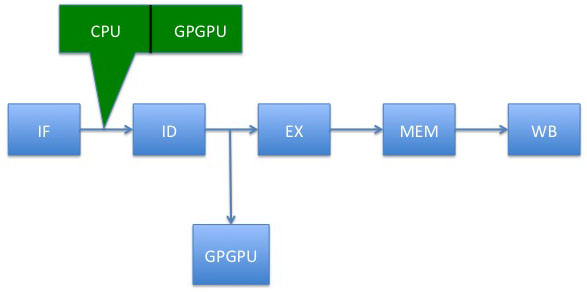
\includegraphics[scale=0.75]{diagrams/diag1.jpg}
\caption{Illustration of the heterogenous pipeline}
\end{figure}


\section*{Arbitration with the GPGPU}
\addcontentsline{toc}{section}{Arbitration with the GPGPU}

At first glance, it seems that the GPGPU should be treated like a peripheral component that can be locked down by running threads. However, that is not truly designing a heterogenous architecture. The best way to manage this different component would be to think of it as an additional CPU and give that problem to the operating system. As the different classes of programs were outlined previously, giving the operating system arbitration control over the GPGPU does not seem that challenging. The operating system would need to know when processes require the CPU vs. the GPGPU. 









